\section{模型训练过程和测试过程}
为确保回归模型高效收敛并输出可靠的拟合结果,本实验构建了“预处理-训练-可视化”三位一体的完整训练流程,从数据准备到结果呈现的各环节设计如下:

\subsection{训练前的数据预处理:必要性与操作逻辑}
数据预处理是模型训练的\textbf{前置必要步骤},其有效性直接决定梯度下降算法的稳定性与收敛效率。原始输入特征矩阵$\boldsymbol{X}$中,不同特征往往存在量纲差异(例如“样本温度”特征取值范围为$[0, 100]$,“样本湿度”特征取值范围为$[0, 1]$)。若直接使用原始数据训练,会导致损失函数的梯度分布严重失衡——即使设置常规学习率(如$\eta=0.01$),也可能出现参数更新幅度过大、损失值震荡不收敛,甚至梯度爆炸等“意想不到的错误”。

因此,训练前需对$\boldsymbol{X}$执行标准化操作(基于各特征的均值$\overline{x}_i$与标准差$\sigma_i$),将所有特征映射到相近的数值区间。具体标准化公式参考前文定义:
\[
x_{i,j}^{\text{标准化}} = \frac{x_{i,j} - \overline{x}_i}{\sigma_i}
\]
其中$x_{i,j}$为原始特征值,$x_{i,j}^{\text{标准化}}$为标准化后的特征值。通过该操作,可使各特征的均值趋近于0、标准差趋近于1,为梯度下降的稳定迭代提供数据基础。

\subsection{迭代训练逻辑与收敛控制}
模型训练基于前文定义的梯度下降函数(线性回归/岭回归/Lasso回归),核心训练逻辑与终止条件设计如下:
\begin{itemize}
    \item[1] \textbf{迭代触发与参数更新}:模型启动后,每轮训练均按“预测值计算→误差求解→梯度计算→参数更新”的流程执行(对应公式$\hat{y}=X\cdot\theta$、$e=\hat{y}-y$、$\nabla J(\theta)=\frac{1}{m}X^T\cdot e$、$\theta=\theta-\eta\cdot\nabla J(\theta)$),若为岭回归或Lasso回归,额外执行对应正则化修正(L2正则化$\theta_i=\theta_{\text{temp},i}-\eta\cdot\alpha\cdot\theta_{\text{temp},i}$或L1正则化$\theta_i=\theta_{\text{temp},i}-\eta\cdot\alpha\cdot\text{sign}(\theta_{\text{temp},i})$)。
    \item[2] \textbf{收敛控制策略}:设置双重终止条件以平衡训练效率与结果精度:
    \begin{itemize}
        \item[1] 最大迭代次数限制:将训练轮次上限设为1000次,避免因梯度长期小幅波动导致训练耗时过长;
        \item[2] 梯度范数阈值:当梯度向量的L2范数$\|\nabla J(\theta)\| < 10^{-6}$时,判定参数更新已趋于稳定,提前终止训练。
    \end{itemize}
\end{itemize}

实验验证表明,在标准化数据支撑下,即使触发最大迭代次数(1000次),模型也能基本达成预期的拟合效果,满足后续分析需求。

\subsection{实时可视化与结果呈现}
为直观追踪训练过程中参数变化与模型拟合效果的关联,实验设计了\textbf{实时可视化机制}:基于梯度下降的每轮参数更新结果,系统每1ms自动生成并刷新一次训练图像。该图像并非直接展示高维特征空间数据,而是将输入特征与预测结果投影到“所选标签对应的投影平面”上——通过降维呈现,可清晰观察样本点在训练过程中与拟合直线(或超平面)的相对位置变化,间接反映模型拟合精度的提升趋势。

典型的训练过程可视化结果如图\ref{fig:train_process}所示,该图记录了某轮Lasso回归训练中,样本投影点与拟合直线的动态适配过程,可直观判断模型是否存在过拟合、欠拟合或收敛停滞等问题。

\begin{figure}[!htb]
    \centering
    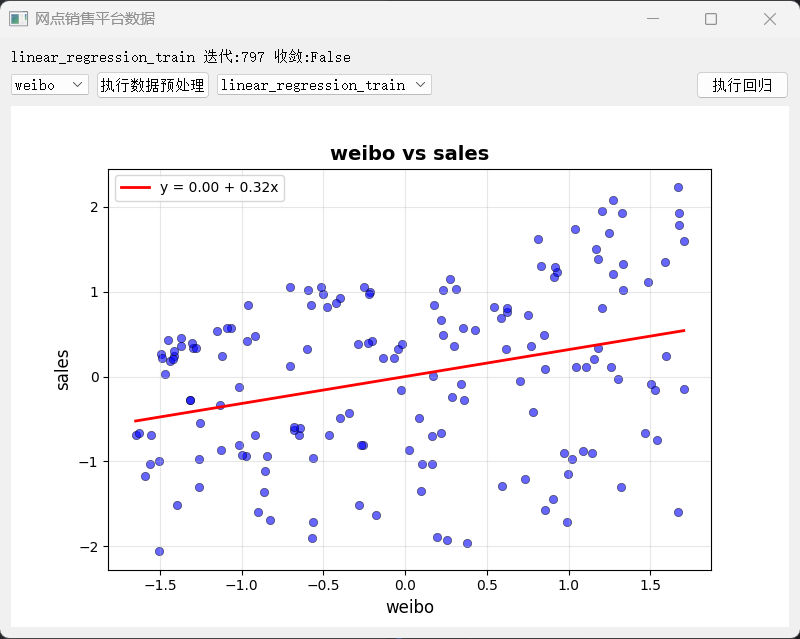
\includegraphics[width=0.70\textwidth]{./figures/train.png}
    \caption{模型训练过程可视化(投影平面图像)}
    \label{fig:train_process} % 图表标签,用于后文引用
\end{figure}

\subsection{训练流程启动与模型选择}
实际训练时,用户仅需在实验脚本中指定两项核心参数即可启动流程:
\begin{itemize}
    \item[1] 回归方法选择:根据任务需求(如是否需特征选择、是否需抑制过拟合),选择“线性回归”“岭回归”或“Lasso回归”;
    \item[2] 超参数确认:确认学习率$\eta$(默认0.01)、正则化强度$\alpha$(岭回归/Lasso回归,默认0.5)等超参数取值。
\end{itemize}

参数配置完成后,系统将自动执行“数据预处理→迭代训练→实时可视化”的全流程,直至满足收敛条件后输出最终模型参数$\theta$与训练日志。

\subsection{MSE评估训练结果}
完成前置处理后,基于测试集真实标签$y_{\text{true}}$与反归一化后的预测值$\hat{y}$,计算MSE的公式为:
\[
\text{MSE} = \frac{1}{m_{\text{test}}} \sum_{k=1}^{m_{\text{test}}} \left( \hat{y}_k - y_{\text{true},k} \right)^2
\]
其中$\hat{y}_k$为第$k$个测试样本的预测值,$y_{\text{true},k}$为第$k$个测试样本的真实标签,$m_{\text{test}}$为测试集样本总数。

在实验代码中,该公式通过np.mean((y\_pred-y\_true)**2)实现,计算完成后会输出预测值$\hat{y}$、标签标准差$\sigma_y$、标签均值$\overline{y}$与真实标签$y_{\text{true}}$在控制台上,并在图形化界面中展示出mse结果,便于后续误差溯源与结果分析。

\begin{figure}[!htb]
    \centering
    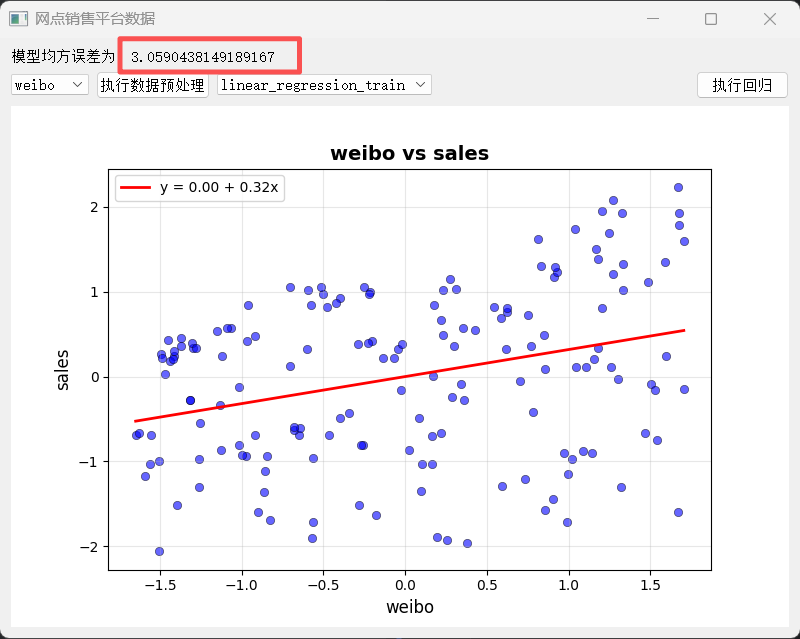
\includegraphics[width=0.70\textwidth]{./figures/mse.png}
    \caption{模型训练过程可视化(投影平面图像)}
    \label{fig:mse_process} % 图表标签,用于后文引用
\end{figure}